\section{Aufbau}
\label{sec:Aufbau}
\begin{figure}
	\centering
	\caption{Der schematische Aufbau des Michelson-Interferometer \cite{V401}.}
	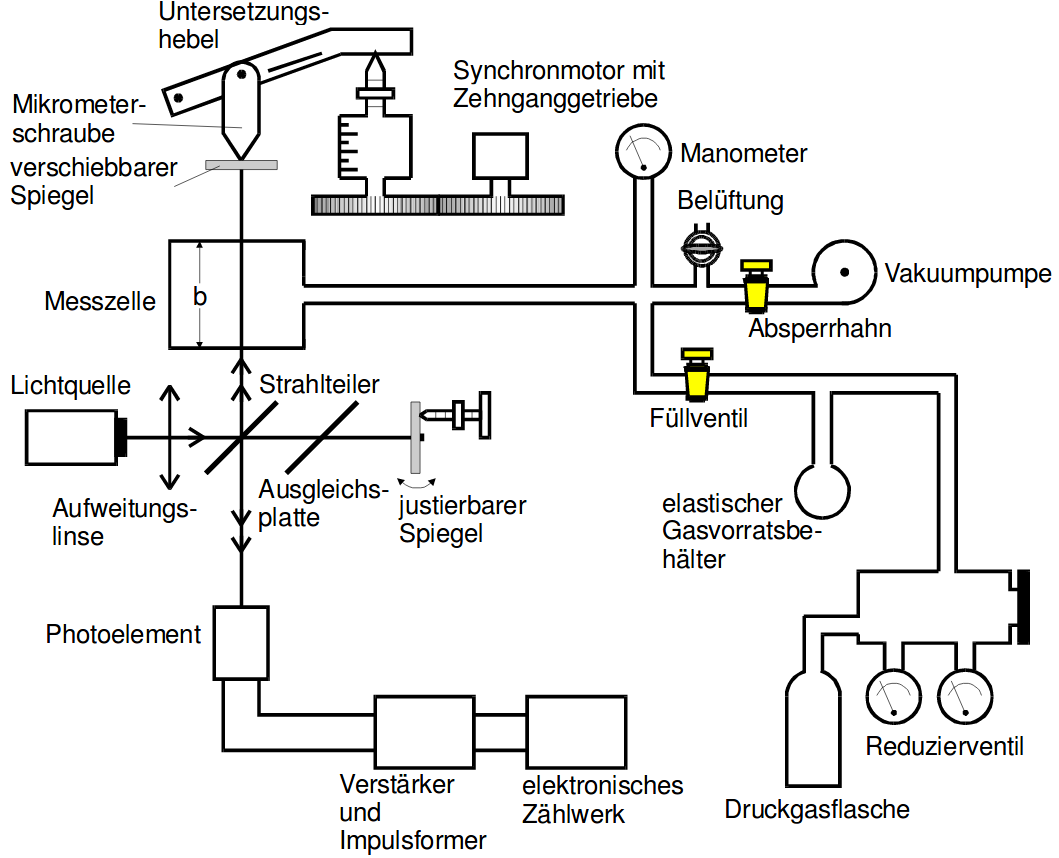
\includegraphics[width=\linewidth-150pt,height=\textheight-150pt,keepaspectratio]{content/aufbau.png}
	\label{fig:aufbau}
\end{figure}
Der Messaufbau besteht im Kern aus dem in der Theorie beschriebenen Konzept der
Interferenz zweier kohärenter Lichtstrahlen. Hierzu wird der Strahl eines Helium-Neon-Lasers
über eine Aufweitungslinse auf einen halbdurchlässigen Spiegel gelenkt, welcher den Strahl in zwei neue Strahlen aufteilt.
Ein Strahl läuft über eine Ausgleichsplatte auf einen justierbaren Spiegel und wieder zurück.
Der andere Strahl läuft durch eine Messzelle, in welcher der vorherrschende Luftdruck modifiziert werden kann.
Hierzu wird eine handbetriebene Vakuumpumpe mit integriertem Manometer verwendet.
Auch dieser Lichtstrahl trifft anschließend auf einen Spiegel und wird wieder zurück reflektiert.
Der Spiegel lässt sich über eine Mikrometerschraube und einen untersetzen Synchronmotor langsam verschieben.
Beide Strahlen kommen beim halbdurchlässigen Spiegel zur Interferenz und treffen anschließend auf ein Photoelement.
Über einen Verstärker und einen Impulsformer kann anschließend die Zahl der auftretenden Interferenzmaxima gezählt werden.
